%%%%%%%%%%%%%%%%%%%%%%%%%%%%%%%%%%%%%%%%%%%%%%%%%%%%%%%%%%%%%%%%%%%%%%%%%%%%%%%%
%	TRABAJO: Proyecto Integrador
%		Titulo: 	Desarrollo de IP cores con procesamiento de Redes de Petri 	
%					Temporales para sistemas multicore en FPGA					
%		Autores:	Juli�n Nonino												%					Carlos Renzo Pisetta										%		Director:	Orlando Micolini											
%%%%%%%%%%%%%%%%%%%%%%%%%%%%%%%%%%%%%%%%%%%%%%%%%%%%%%%%%%%%%%%%%%%%%%%%%%%%%%%%

% Path im�genes: ./marco_teorico/redes_de_petri/img
% Nombre predeterminado im�genes: petrixx
%	xx es el numero de imagen

\section{Extensiones de las Redes de Petri}
	\label{sec:extensiones}

	Las Redes de Petri analizadas hasta el momento, pueden ser extendidas agregando arcos inhibidores para considerar la ausencia de tokens como condici�n de sensibilizaci�n de una transici�n (\textbf{\emph{Redes de Petri con Arcos Inhibidores}}), marcas de tiempo para determinar intervalos en los cuales una transici�n puede ser disparada (\textbf{\emph{Redes de Petri con Tiempo}}), o valores de duraci�n en las transiciones(\textbf{\emph{Redes de Petri Temporizadas}}), probabilidades de disparo de transiciones (\textbf{\emph{Redes de Petri Estoc�sticas}}) o cualquier combinaci�n entre ellas.
	
	En la Figura \ref{fig:Petri14}, extra�da del libro \cite{diaz_petri}, se observa la evoluci�n de estas extensiones. Se encuentran marcadas, aquellas que se analizar�n en este trabajo. Las \emph{Redes de Petri con Arcos Inhibidores} est�n incluidas dentro de �tem \emph{Place-transition Petri nets 1962, 1969}.
		
	\begin{figure}[H]
		\centering
		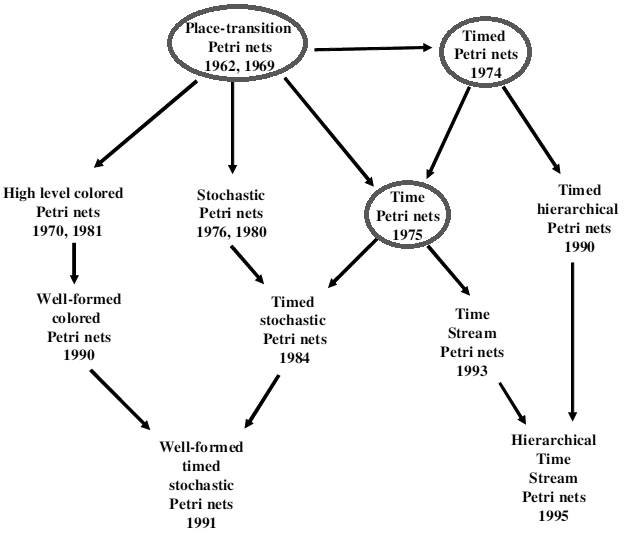
\includegraphics[width=1\linewidth]{./marco_teorico/redes_de_petri/img/Petri14}
		\caption{Extensiones de las Redes de Petri}
		\label{fig:Petri14}
	\end{figure}	
		